\section{Results}
\note{This section includes all results of running the simulation, with reports of expected time to detection being primary focus}


\note{from c\&B analysis of sequential decision making}
\note{Consider the following setting, where a single stationary tar-get is possibly located in a10×10 search region that is depicted in Fig. 5. The initial aggregate beliefB(0) is distributed among theC= 100 cells,  where  the  height  of  the  bars  in  each  cell represents the individual cell belief values, i.e., the probabilityp0cthat the target is present in a given cell, i.e.,c in {1,...,C} . SupposeB(0) = 0.75 ,  which  corresponds  to  an  initial  likeli-hood of 75\% that the target is truly present inA at the beginning of the search process. We examine the evolution of the search decision employing the different search strategies that are presented in the previous section. The search problem parameters that are used for the simulation studies, which are presented in this section, are tabu-lated in Table I. Simulations were allowed to run to completion (i.e., a decision was made), and statistics were calculated over N= 10 000 simulation replications. The values for the detec-tion errors, i.e.,alpha and beta , were chosen to reflect a representative sensor, such as a visual camera that provides aerial imagery in an outdoor and cluttered environment, which could be further calibrated empirically, e.g., by the sensor’s receiver operating characteristic (ROC) curve. Fig.  6  illustrates  the  evolution  of  the  belief  map  as  a search  agent  that  employs  the  myopic  search  strategy  thatmoves through the search region for the given search problem parameters. The searcher attempts to inspect or “clear” cells with the highest cell belief values, which, for the example bimodal belief distribution, requires visiting one peak followed by explo-ration of the other. Note that false-positive and false-negative detections  occur  throughout  the  search  process,  although  the searcher eventually arrives at the true location of the target and correctly terminates the search}


note{From C\&B Analysis of sequential decision-making using prob. search. Consider a bounded discretized search areaA , which is de-fined byC disjoint cells. This discrete representation can charac-terize numerous environment types of diverse spatial scale, such as open areas that are relevant to maritime search operations, cluttered regions, such as obstacle-filled arenas, or structured environments, such as rooms and hallways in a building. Other factors, which include the geometry and extent of the searcher’s sensor footprint, and the size of the sought object, or other op-erational considerations (e.g., existing coordinates or reference systems) can also govern the specific cellular decomposition of the search area}

\note{More general sensor models that account for additional spatial and/or temporal dependences be-cause  of  clutter  (indoor)  or  terrain  and  atmosphere  (outdoor) can  be  constructed  (e.g.,$\alpha$ s(k),kand $\beta$ s(k),k )  but  is  deferred for future study}


\note{In other words, the greater hindrance to deciding that a target is present in the search cell is the false-positive detection probabil-ity, since false alarms tend to prevent the searcher from “trust-ing” its positive observation. In contrast, if the missed detection probability is high, then the searcher cannot declare the search cell empty of the target with high confidence without expending multiple observations in the c}


The results presented in this section are generated by running monte carlo simulations, since finding a close-form solution to the expected time to decision (ETTD) is not readily available in the general case \cite{Chung2012AnalysisStrategies}. The results of running the target search depends on a number of factors: the prior belief distribution of each agent, the Type \Romannum{1} and Type \Romannum{2} error rates, the search strategies employed by the agents and . In order to evaluate the performance of the system that we have developed, we focus on the mostly commonly reported metrics in the literature, which are all related to the distribution of time to decision \cite{Chung2012AnalysisStrategies}, \cite{Waharte2010ProbabilisticUAVs}, \cite{Waharte2010SupportingUAVs}, \cite{Lau2007OptimalEnvironments}. 


\begin{table}[h!]
  \centering
  \begin{tabular}{ | c | m{5.2cm} | }
    \hline
     & Parameters/Statistics \\
    \hline
    
    %single UAV
    \begin{minipage}[c][45mm][c]{.6\textwidth}
      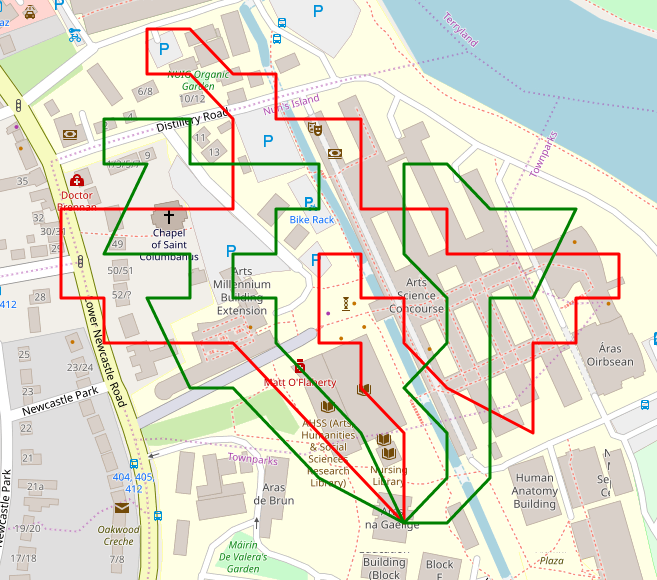
\includegraphics[width=\linewidth, height=43mm]{Chapters/MultiAgentCoverage/MultipleTravellingSalesman/Figs/ORToolsSolns/Example1.PNG}

    \end{minipage}
    &
    \small
    \begin{tabular}{m{10mm}|m{11mm} m{11mm}}
        & Search Strategy & UAV 2\\
        \hline
        Speed& 4 & 2 \\
        T.T.S & 0.5 & 0.5 \\
        Color & Red & Green \\
        \hline
        Dist.& 1813 & 1813 \\
        Time& 1410 & 1600 \\
    \end{tabular}
    \normalsize
    \\
    \hline
    %single UAV
    \begin{minipage}[c][45mm][c]{.6\textwidth}
      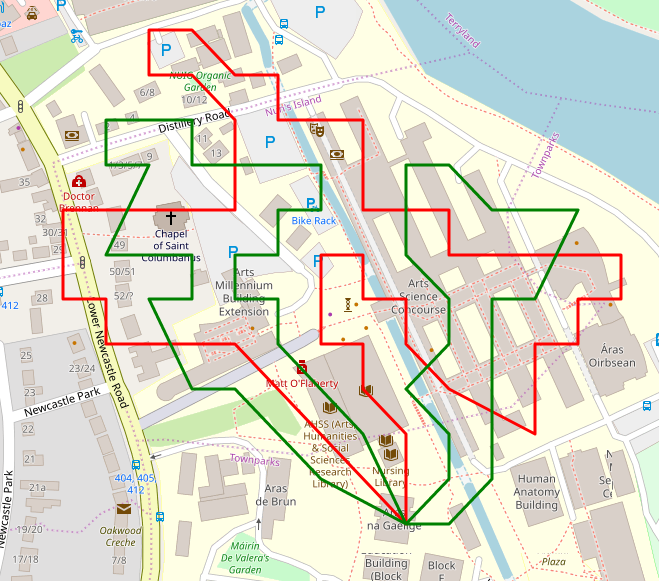
\includegraphics[width=\linewidth, height=43mm]{Chapters/MultiAgentCoverage/MultipleTravellingSalesman/Figs/ORToolsSolns/Example2.PNG}

    \end{minipage}
    &
    \small
    \begin{tabular}{m{10mm}|m{11mm} m{11mm} }
        & UAV 1 & UAV 2\\
        \hline
        Speed& 1 & 1 \\
        T.T.S & 0.5 & 0.5 \\
        Color & Red & Green \\
        \hline
        Dist.& 1961 & 2141 \\
        Time& 3423 & 3423 \\
    \end{tabular}
    \normalsize
    \\
    \hline
    
    %single UAV
    \begin{minipage}[c][45mm][c]{.6\textwidth}
      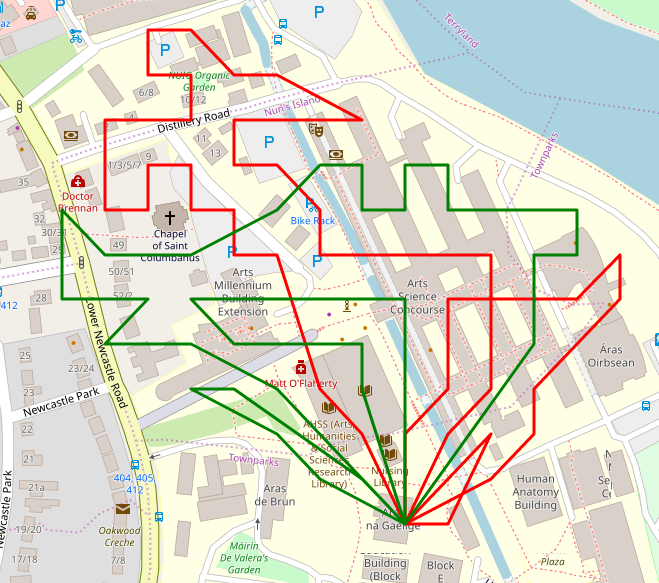
\includegraphics[width=\linewidth, height=43mm]{Chapters/MultiAgentCoverage/MultipleTravellingSalesman/Figs/ORToolsSolns/Example3.PNG}

    \end{minipage}
    &
    \small
    \begin{tabular}{m{10mm}|m{11mm} m{11mm}}
        & UAV 1 & UAV 2\\
        \hline
        Speed& 1 & 1 \\
        T.T.S & 2 & 2 \\
        Color & Red & Green \\
        \hline
        Dist.& 2142 & 2150 \\
        Time& 3462 & 3462 \\
    \end{tabular}
    \normalsize
    \\
    \hline
    
    %single UAV
    \begin{minipage}[c][45mm][c]{.6\textwidth}
      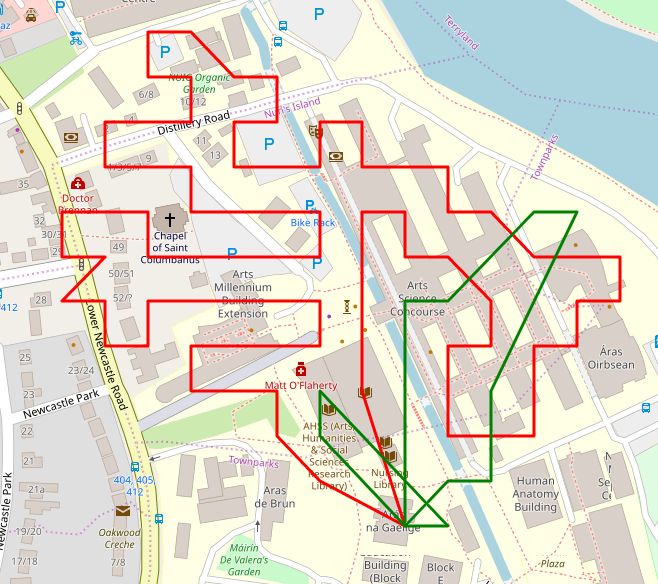
\includegraphics[width=\linewidth, height=43mm]{Chapters/MultiAgentCoverage/MultipleTravellingSalesman/Figs/ORToolsSolns/Example4.PNG}

    \end{minipage}
    &
    \small
    \begin{tabular}{m{10mm}|m{11mm} m{11mm}}
        & UAV 1 & UAV 2\\
        \hline
        Speed& 8 & 1 \\
        T.T.S & 1 & 1 \\
        Color & Red & Green \\
        \hline
        Dist.& 2638 & 870 \\
        Time& 1410 & 1600 \\
    \end{tabular}
    \normalsize
    \\
    \hline

  \end{tabular}
  \caption{Results of applying solution found with OR-Tools solver. T.T.S = Time to sample, Dist. = Distance}\label{table:ORToolsResults}
\end{table}

We report on the expected time to decision, the variance in time to decision, the precision and recall and 